%	To produce Postscript and PDF:
%    latex template; latex template; 
%    dvips -o template.ps template; ps2pdf template.ps
\documentclass[a4paper,11pt]{article}
\usepackage{mathptmx}
%\usepackage{newtxmath}   not available ? 
%\usepackage{newtxtext} []  not available ?
\usepackage[margin=28mm]{geometry}% <-------- CHANGE HERE for the global margins
\usepackage[T1]{fontenc}    % Check that ÖÄÅöäå come out ok!
\usepackage[utf8]{inputenc}
\usepackage{graphicx}
\usepackage{url} 
\usepackage{parskip}
\usepackage{listings} % for code snippets
\usepackage{authblk}
\usepackage[nobottomtitles]{titlesec}
\linespread{1.1}
\usepackage[bottom]{footmisc}
\usepackage[title]{appendix}
\usepackage{perpage} %the perpage package
\MakePerPage{footnote} %the perpage package command
\usepackage{varioref} %for \vref
\usepackage{enumitem}
\usepackage{wrapfig}
\usepackage[table]{xcolor} % for table colors (gray)
\usepackage{caption}
\usepackage{pdfpages}
% for printing current date and time on compile time
\usepackage{fancyhdr}
\usepackage[yyyymmdd,hhmmss]{datetime}
\pagestyle{fancy}
%
% should not USE  ? 
%\setlength{\parindent}{10mm} % Do not indent the 1st line of a paragraph.
%\setlength{\parskip}{20mm}   % Add space between paragraphs.

% defined new environments
\newenvironment{filecode}[1][]
  {\minipage{\linewidth}% \begin{filecode}[#1]
   \lstset{basicstyle=\ttfamily\footnotesize,#1}}
  {\endminipage}% \end{filecode}

\newenvironment{note}[1]
  {
  \vspace{1em}\hspace{1.5em}
  \hbox{%
  \vrule\hspace{.5em}\parbox{.9\textwidth}%
  {
  \textbf{Note:}
  #1
  }}}
  {\vspace{1em}}

\renewenvironment{abstract}
{\itshape \small
  \begin{center}
  \bfseries \abstractname\vspace{-.5em}\vspace{0pt}
  \end{center}
  \list{}{
    \setlength{\leftmargin}{1.5cm}%
    \setlength{\rightmargin}{\leftmargin}%
  }%
  \item\relax}
{\endlist}


% defines my code style
\usepackage{color}
\usepackage{courier}

\definecolor{dkgreen}{rgb}{0,0.6,0}
\definecolor{gray}{rgb}{0.5,0.5,0.5}
\definecolor{mauve}{rgb}{0.58,0,0.82}

\lstset{frame=tb,
  language=Java,
  aboveskip=3mm,
  belowskip=3mm,
  showstringspaces=false,
  columns=flexible,
  basicstyle={\scriptsize\ttfamily},
  numbers=left,
  numbersep=4pt,
  numberstyle=\scriptsize\color{gray},
  keywordstyle=\color{blue},
  commentstyle=\color{dkgreen},
  stringstyle=\color{mauve},
  moredelim=[s][\color{gray}]{@}{\ },
  breaklines=true,
  breakatwhitespace=true,
  tabsize=2
}

\lstdefinelanguage{JavaScript}{
  keywords={typeof, new, true, false, catch, function, return, null, catch, switch, var, if, in, while, do, else, case, break},
  keywordstyle=\color{blue},
  ndkeywords={class, export, boolean, throw, implements, import, this},
  ndkeywordstyle=\color{gray},
  identifierstyle=\color{black},
  sensitive=false,
  comment=[l]{//},
  morecomment=[s]{/*}{*/},
  commentstyle=\color{dkgreen}\ttfamily,
  stringstyle=\color{blue}\ttfamily,
  morestring=[b]',
  morestring=[b]"
} 

% title variable definition
\newcommand{\mahtitle}{Assortativity of k-NN graphs}

% Save some paper by stuffing more text on each page:
% A4: 210mm x 297mm, approximately 35 mm margins on every side.
\addtolength{\topmargin}{-2mm}    
\addtolength{\textheight}{2mm}    
%\addtolength{\oddsidemargin}{-10mm} 
%\addtolength{\textwidth}{14mm}     

% This creates the header.
%\makeatletter
%\renewcommand{\@oddhead}
%{\fontsize{10}{12}\selectfont \hfill \mahtitle \hfill }
%\makeatother

\renewcommand{\Authfont}{\Large\normalfont}
\renewcommand{\Affilfont}{\large\itshape}


% This creates the header.
\setlength{\headheight}{14pt}
\fancyhf[HL]{Built: \today\ at \currenttime}
\fancyhf[HC]{\mahtitle}
\fancyhf[HR]{}

\begin{document}

%============================================================
% title
\label{Title} 
\title{\vspace{1pc} \mahtitle \vspace{4pc}}
\author{Patryk Małek \vspace{-0.7pc}}
\affil{
        University of Novi Sad\\
        Faculty of Sciences\\
        malekpatryk@gmail.com
      }
\date{}
%\date{\today}         % Do not print the date on the final paper!
\maketitle
% prevents page numbering on this page
\thispagestyle{empty}

%============================================================

\vspace{6pc}
\centerline{

\includegraphics[width=0.35\textwidth,height=0.35\textheight,keepaspectratio]{NoviSadLogoGray.jpg}
}
\vspace{8pc}

\clearpage
\begin{abstract}
\label{Abstract}
Most social, biological or technological networks which we describe as complex networks exhibit substantial nontrivial topological features, with some patterns of connections between their nodes that are not purely irregular.
Such features include amongst others assortativity or disassortativity of nodes.
Assortativity is the tendency of nodes to connect to other nodes that are similar to them.
Highly dimensional, real-world datasets tend to contain hubs – instances whose in-degree (the number of incoming links attached to a node) is extremely high.

This paper investigates investigates assortativity of k-NN graphs constructed from real-world high-dimensional datasets by means of trying to find correlation of $k$ parameter of k-NN graphs to graphs' assortativity index.
After introducing the notion of k-NN graphs general problem definition is given regarding relation of $k$ parameter and graph's assortativity coefficient (also called Pearson correlation coefficient) in high dimensional datasets.
With positive assortative index $(0, 1>$, nodes tend to connect to other nodes that are similar.
With negative assortative index $<-1, 0$, nodes tend to connect to nodes that are different (have different degrees).
Values close to $0$ indicate no tendency of nodes to connect to any other particular nodes (random connections).
In this paper analysis of exemplar high-dimensional real-world datasets is given, basing on analyzing tool implemented for project's needs.
The discovered rules whether k-NN graphs representing real-world data are assortative, disassortative or show no degree correlations are given in the results section.
\end{abstract}

%============================================================

\clearpage
\tableofcontents

%============================================================

\clearpage
\section{Introduction} 
Intention of this research paper is to define whether there exists correlation between in-degrees of connected nodes (that is number of connections going in the nodes) in kNN graphs and their out degrees, which is denoted here as parameter $k$, in real world datasets.
Reserach results may be helpful for researchers that would like investigate properties of networks created from real world, high dimensional datasets.
To solve the problem a solution software has been implemented to help with creating kNN graphs and visualizing the results.
\subsection{Background}
\subsubsection{K Nearest Neighbor graphs}
K nearest neighbor graph for a set of $n$ objects $P$ in a metric space (e.g., for a set of points in the plane with Euclidean distance) is a directed graph with $P$ being its vertex set and with a directed edge from $p$ to $q$ whenever $q$ is a nearest neighbor of $p$ (i.e., the distance from $p$ to $q$ is no larger than from $q$ to any other object from $P$).
They can show a measure of the correlation between the degree of a node and that of its neighbors.
In many systems strong correlations are observed, and one distinguishes networks into assortative and disassortative.
A network is assortative if large (small) degree nodes tend to be linked with large (small) degree nodes.
Typical examples of assortative networks are social networks~\cite{information_or_social_network}.
A network is disassortative if large (small) degree nodes tend to be linked with small (large) degree nodes.
Biological and technological networks (like the Internet) are examples of disassortative networks.
On a directed graph one distinguishes between indegree (number of edges incoming to a node) and outdegree (number of edges outgoing from a node), so one can also test different types of correlations.

\subsubsection{Pearson Product-Moment correlation coefficient}

The Pearson product-moment correlation coefficient (or Pearson correlation coefficient, for short) is a measure of strength of linear association between two variables and is denoted by $r$ for samples and $\rho$ for populations.
Basically, it indicates how far away all the data points from the dataset are located to the line of best fit (how well the data points fit the new model/line of best fit).
Pearson correlation coefficient, $\rho$, represented with the following formula for populations:

$$ \rho_{X,Y} = \frac{cov(X,Y)}{\sigma_x \sigma_y}$$

Where $\sigma$ is a standard deviation of population and $cov$ is its covariance.
It can be also represented as $r$, using the following formula for samples of size $n$:

$$r = \frac{\sum_{i=1}^{n} (X_i - \bar{X}) (Y_i - \bar{Y}) }
{ \sqrt{\sum_{i=1}^{n} (X_i - \bar{X})^2} \sqrt{\sum_{i=1}^{n} (X_i - \bar{X})^2} }$$

Pearson correlation coefficient can take a range of values from +1 (inclusive) to -1 (inclusive).
A value of 0 indicates that there is no association between the two variables.
A value greater than 0 indicates a positive association; meaning, as the value of one variable increases, so does the value of the other variable.
A value less than 0 indicates a negative association; meaning, as the value of one variable increases, the value of the other variable decreases.

\clearpage
Exemplar Pearson correlation coefficients with graphical representation (and line of best fit) are shown in Figure~\ref{fig:pearson_graph}.

\begin{figure}[h!]
  \centering
  \captionsetup{justification=centering}
    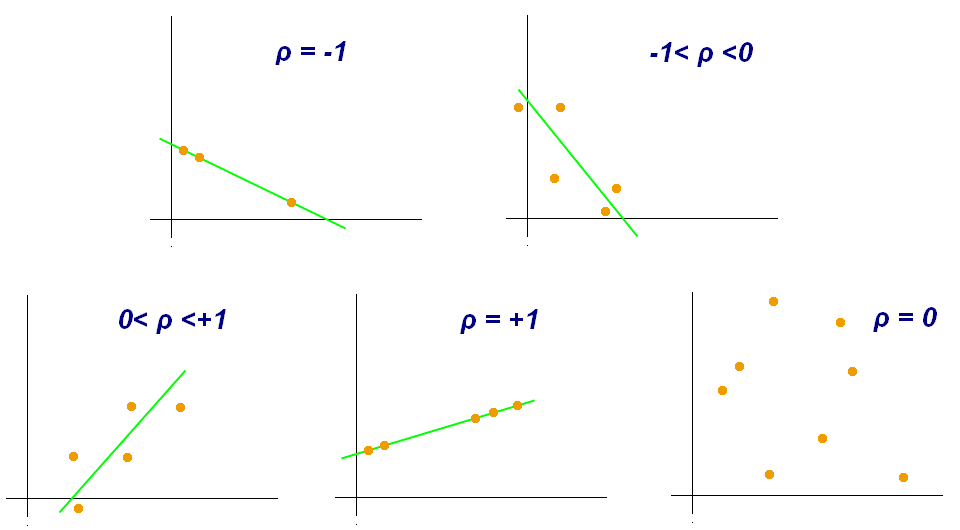
\includegraphics[width=0.8\textwidth]{images/pearson_graphs.png}
  \caption{Graphs showing dependence between graph points, assortativity coefficient and line of best fit.\cite{wiki_pearson}}
  \label{fig:pearson_graph}
\end{figure}

One more thing to note regarding Pearson correlation coefficient is that it does not represent the slope of the line of best fit.
Therefore, if you get a Pearson correlation coefficient of +1 this does not mean that for every unit increase in one variable there is a unit increase in another.
It simply means that there is no variation between the data points and the line of best fit what is illustrated in Figure~\ref{fig:pearson_graph_slope}:

\begin{figure}[h!]
  \centering
  \captionsetup{width=24pc, justification=centering}
    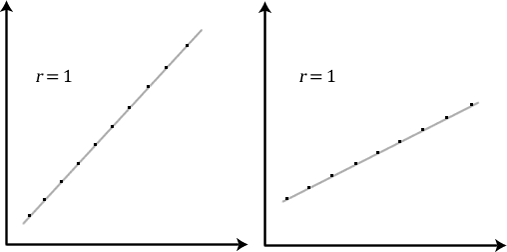
\includegraphics[width=0.55\textwidth]{images/pearson_graphs_slope.png}
  \caption{Graph showing independence of $r$ and slope of the line of best fit.}
  \label{fig:pearson_graph_slope}
\end{figure}

\subsection{Problem definition}
The problem is to define whether there exists relation between parameter $k$ of kNN graph, that is its out-degree (number of outbound connections of each node in the graph) and Pearson correlation coefficient in high dimensional datasets.



%============================================================

\clearpage
\section{Software and technologies used for k-NN graph analysis}
In this chapter, general information about technologies, libraries and programming languages used for creating the solution is given.
In the end of this chapter, the usage of implemented solution is briefly discussed.
\subsection{Used technologies}
%------------------------------------------
\subsubsection{JUNG library}
For creation and representation of graphs and coefficients calculations JUNG library~\cite{jung} has been used.
JUNG(Java Universal Network/Graph Framework) is a software library that provides a common and extendible language for modeling, analysis, and visualization of data that can be represented as a graph or network.

JUNG's \emph{DirectedSparseGraph} has been used as a class being the container for datasets' data.
Datasets' instances has been wrapped in custom \emph{Node} class, having a list of floating point values which were then used for distance calculations.


%------------------------------------------
\subsubsection{Distance algorithm}
For distance algorithm, indicating distance between \emph{Node}s, Euclidean distance algorithm has been implemented.
All values from \emph{Node}'s values list has been squared, summed and then square root of tham sum has been calculated.
The difference between this values of nodes has been used to determine distances between \emph{Node}s.


%------------------------------------------
\subsubsection{Pearson correlation coefficient}
For Pearson correlation coefficient calcalation a class from Apache Common Math library~\cite{apache_common_math} -\emph{org.apache.commons.math3.stat.correlation.PearsonsCorrelation} - has been used.

In this method for each link in the graph we take in-degrees from both of its ends - source node's in-degree and  destination node's in-degree - and then save it in 2 arrays.
After the whole graph has been processed those arrays are then fed to \emph{PearsonsCorrelation} class and the coefficient is calculated with \emph{correlation} method.

\begin{filecode}[label=lst:pearsonCorrelation,caption=Method used for Pearson correlation coefficient calculation.]
  \lstinputlisting{./code/pearsonCorrelation.java}
\end{filecode}

%------------------------------------------
\subsection{Implemented solution}
Implemented solution is a \emph{jar} file with following usage (replace \emph{VERSION} with appropriate version of the \emph{jar} file in possession).

\shellcmd{java -jar knngraphs-VERSION.jar -k K file1.csv [file2.csv ...]}

One can state one or more files (datasets) as shown above which will be used to create kNN graphs, show them and calculate Pearson coefficient vs K graph for each file(dataset).
After launch, user will be asked until what parameter $K$ he wants the program to calculate the graphs (it will start its calcaulations from 1) if it has not been passes in as command line parameter.
After that one can choose whether to show kNN graph for each K ( Warning: it may be RAM and CPU heavy to show graphs for many $K$s) and whether to save Pearson coefficient vs $K$ graph to \emph{.svg} file in the working directory.

Implemented solution's source code has been push onto github repository~\footnote{Patryk Małek, kNN graphs, (2014), GitHub repository,~\url{https://github.com/pmalek/knngraphs}}.

%============================================================

\clearpage
\section{Results}
Using the datasets from University of California Irvine Machine Learning Repository~\cite{uci_datasets}:

\begin{itemize}
\item Cardiac arrythmia dataset~\cite{dataset_cardiac_arythmia}, dataset with 452 instances and a big number of attributes - 279, representing attributes of people having cardiac arrythmia and their organs' states,
\item Handwritten numerals dataset~\cite{dataset_handwritten_numerals}, this dataset consists of features of handwritten numerals ($0$ - $9$) extracted from a collection of Dutch utility maps. 200 patterns per class (for a total of 2,000 patterns) with 64 attributes have been digitized in  binary images and represented in terms of few feature sets that are defined in referenced \emph{arff} file~\cite{dataset_handwritten_numerals},
\item Steel plates faults dataset~\cite{dataset_steel_plates_faults}, describing faults of steel plates like, e.g.: scratches, depth of the scratch, bumps or height of bump. This dataset totals to 1941 instances with 33 attributes each.
\end{itemize}

While using the implemented solution with aforementioned datasets, parameter $k = 30$ has been chosen to calculate the results.

%------------------------------------------
\subsection{Cardiac arrythmia dataset}
\label{subsec:cardiac}
In cardiac arrythmia dataset one can observe assortativity coefficient stabilizing at around $0.31$ indicating assortative mixing.
Between $k$ 1 and 2 we can observe change in assortativity from disassortative to assortative.

Skewness of in-degrees is oscilating around level of $1.4 - 1.5$.
Its level indicates hubs phenomena present in this dataset.

\begin{figure}[h!]
  \centering
  \captionsetup{justification=centering}
    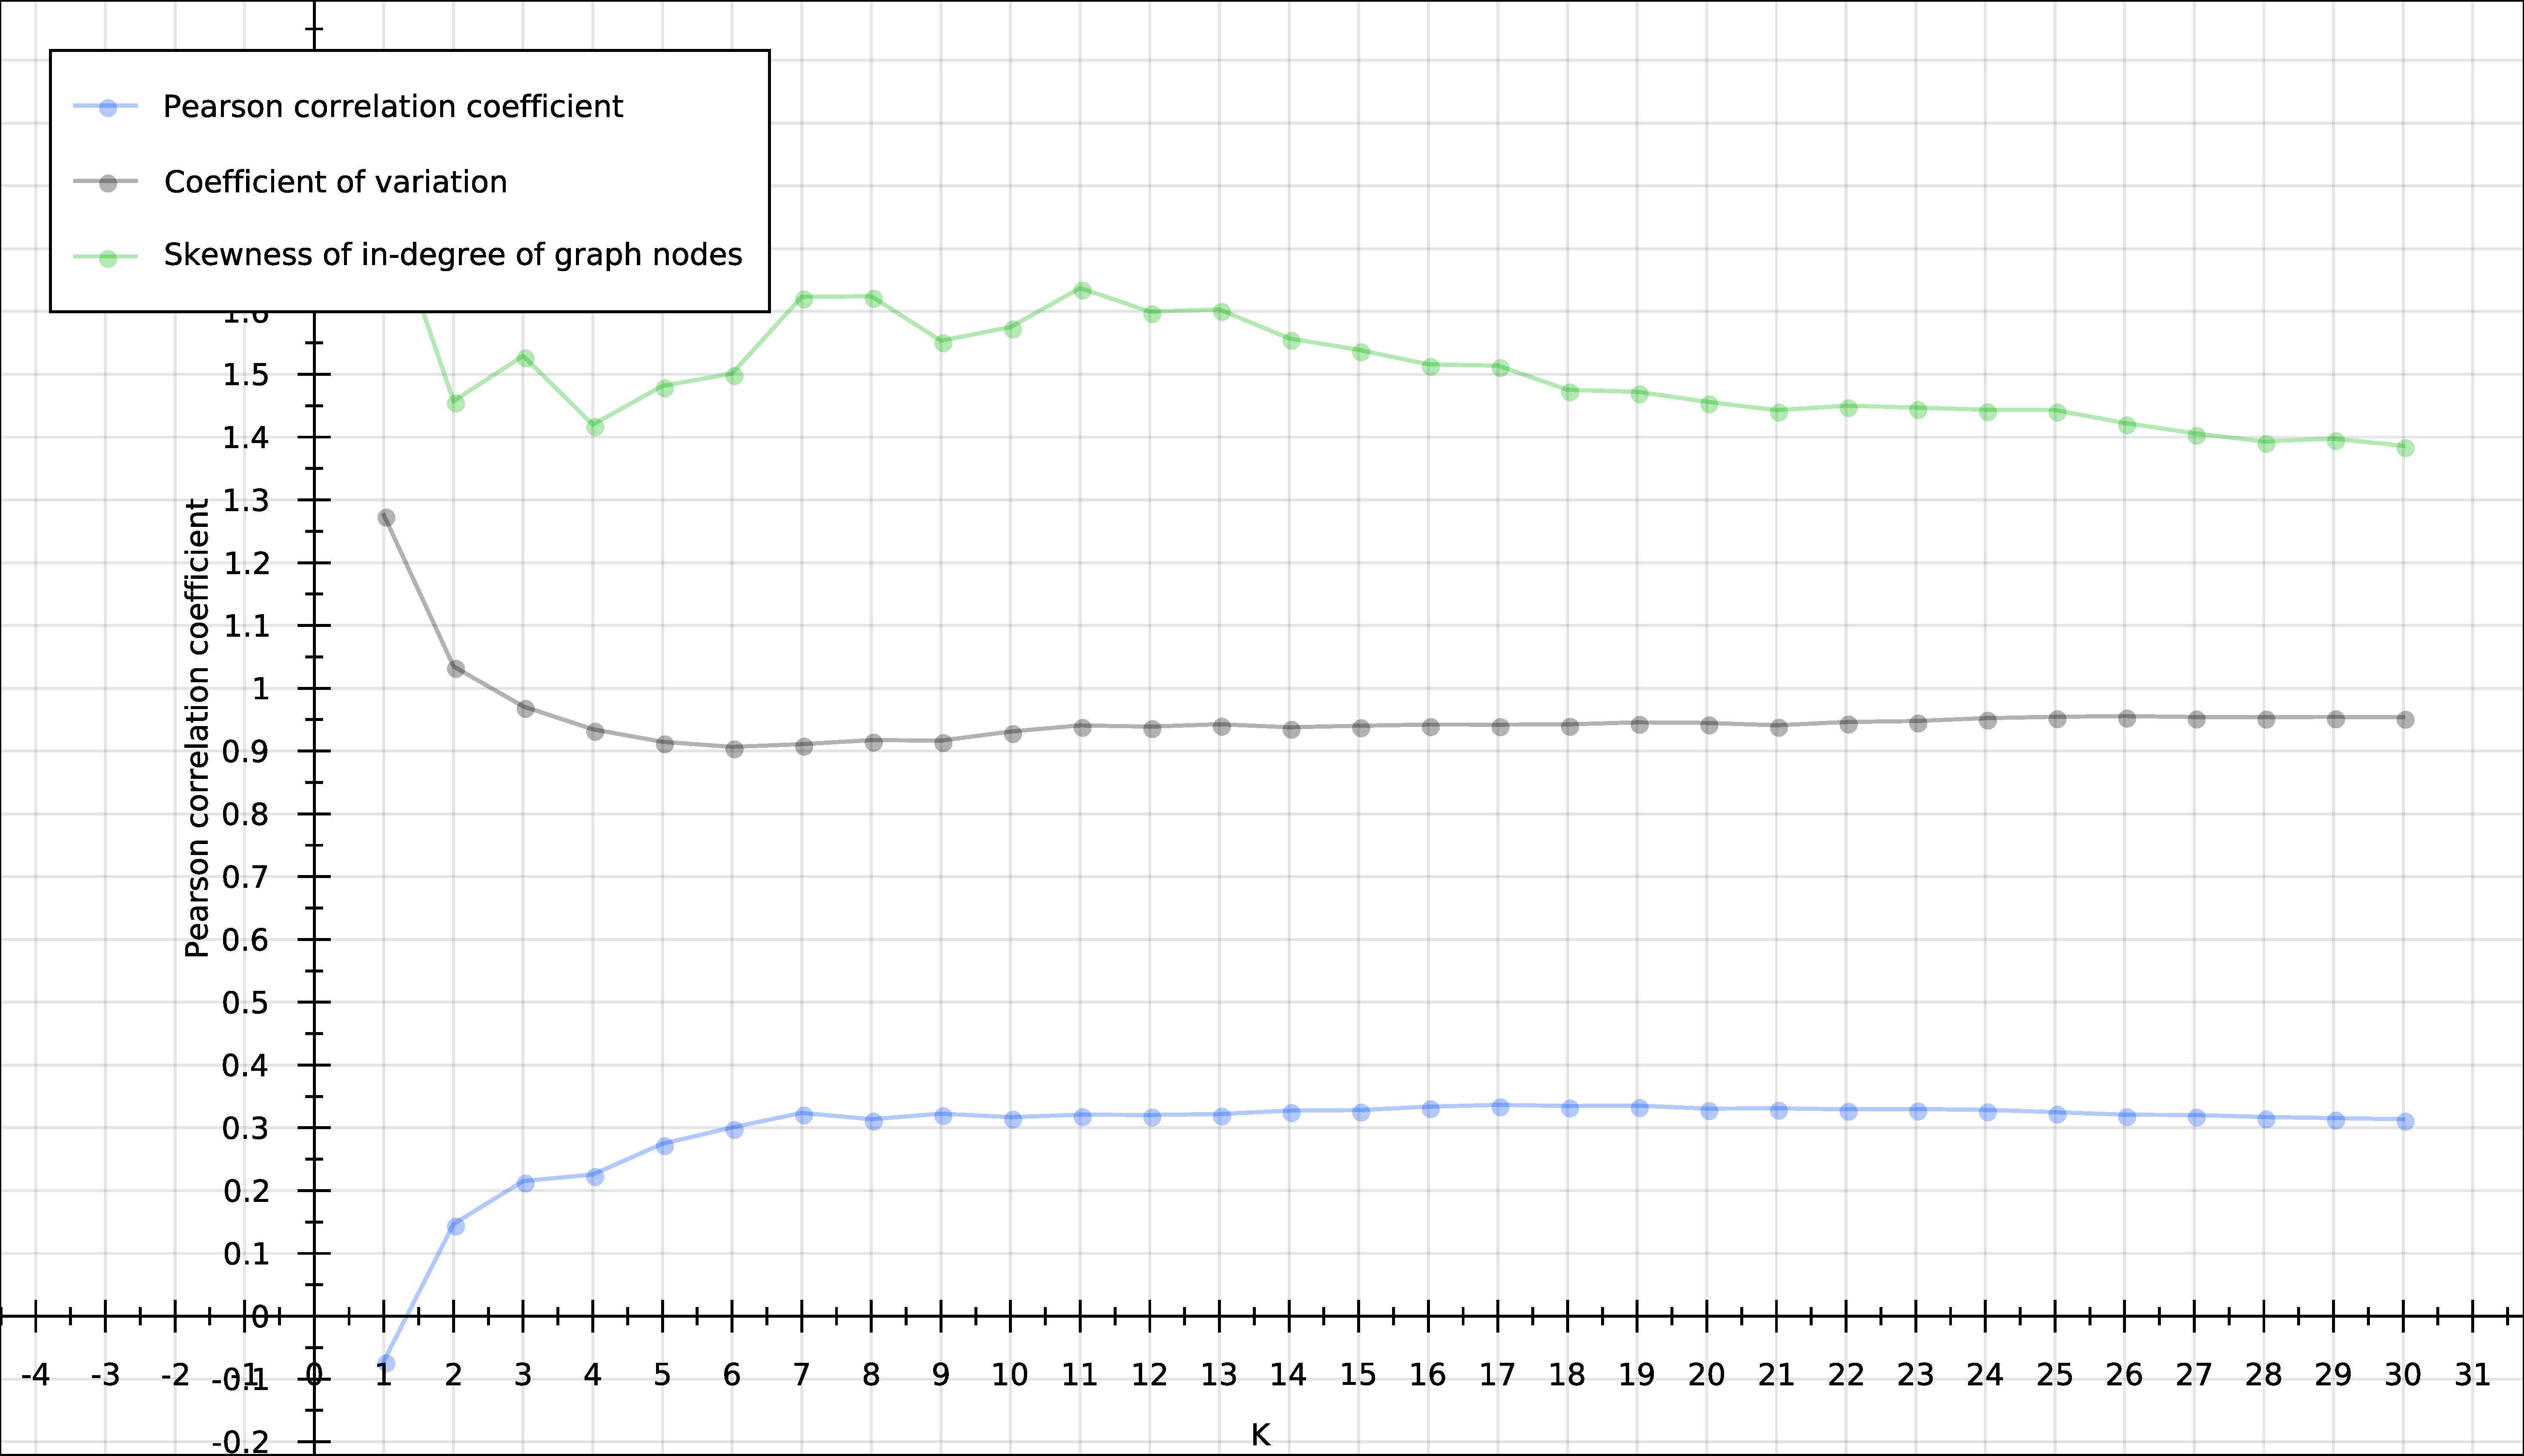
\includegraphics[width=0.95\textwidth]{images/arrythmia_pearson.pdf}
  \caption{Graph of Pearson correlation coefficient, its coefficient of variation and skewness of in-degree of nodes against $K$ parameter for cardiac arrythmia dataset.}
  \label{fig:graph_arrythmia_pearson}
\end{figure}


%------------------------------------------
\subsection{Handwritten numerals dataset}
Handwritten numerals dataset exhibits lower level of stable assortativity index level, at around $0.27$.
In this dataset we can see smaller gap between Pearson correlation coefficient and both skewness and coefficient of variation.

Similarily to cardiac arrythmia dataset in Section~\ref{subsec:cardiac} we can observe a change of assortativity between $k$ 1 and 2 from disassortative to assortative.

Positive skewness of in-degrees proves presence of hubs in kNN graph to be built upon this dataset.

\begin{figure}[h!]
  \centering
  \captionsetup{justification=centering}
    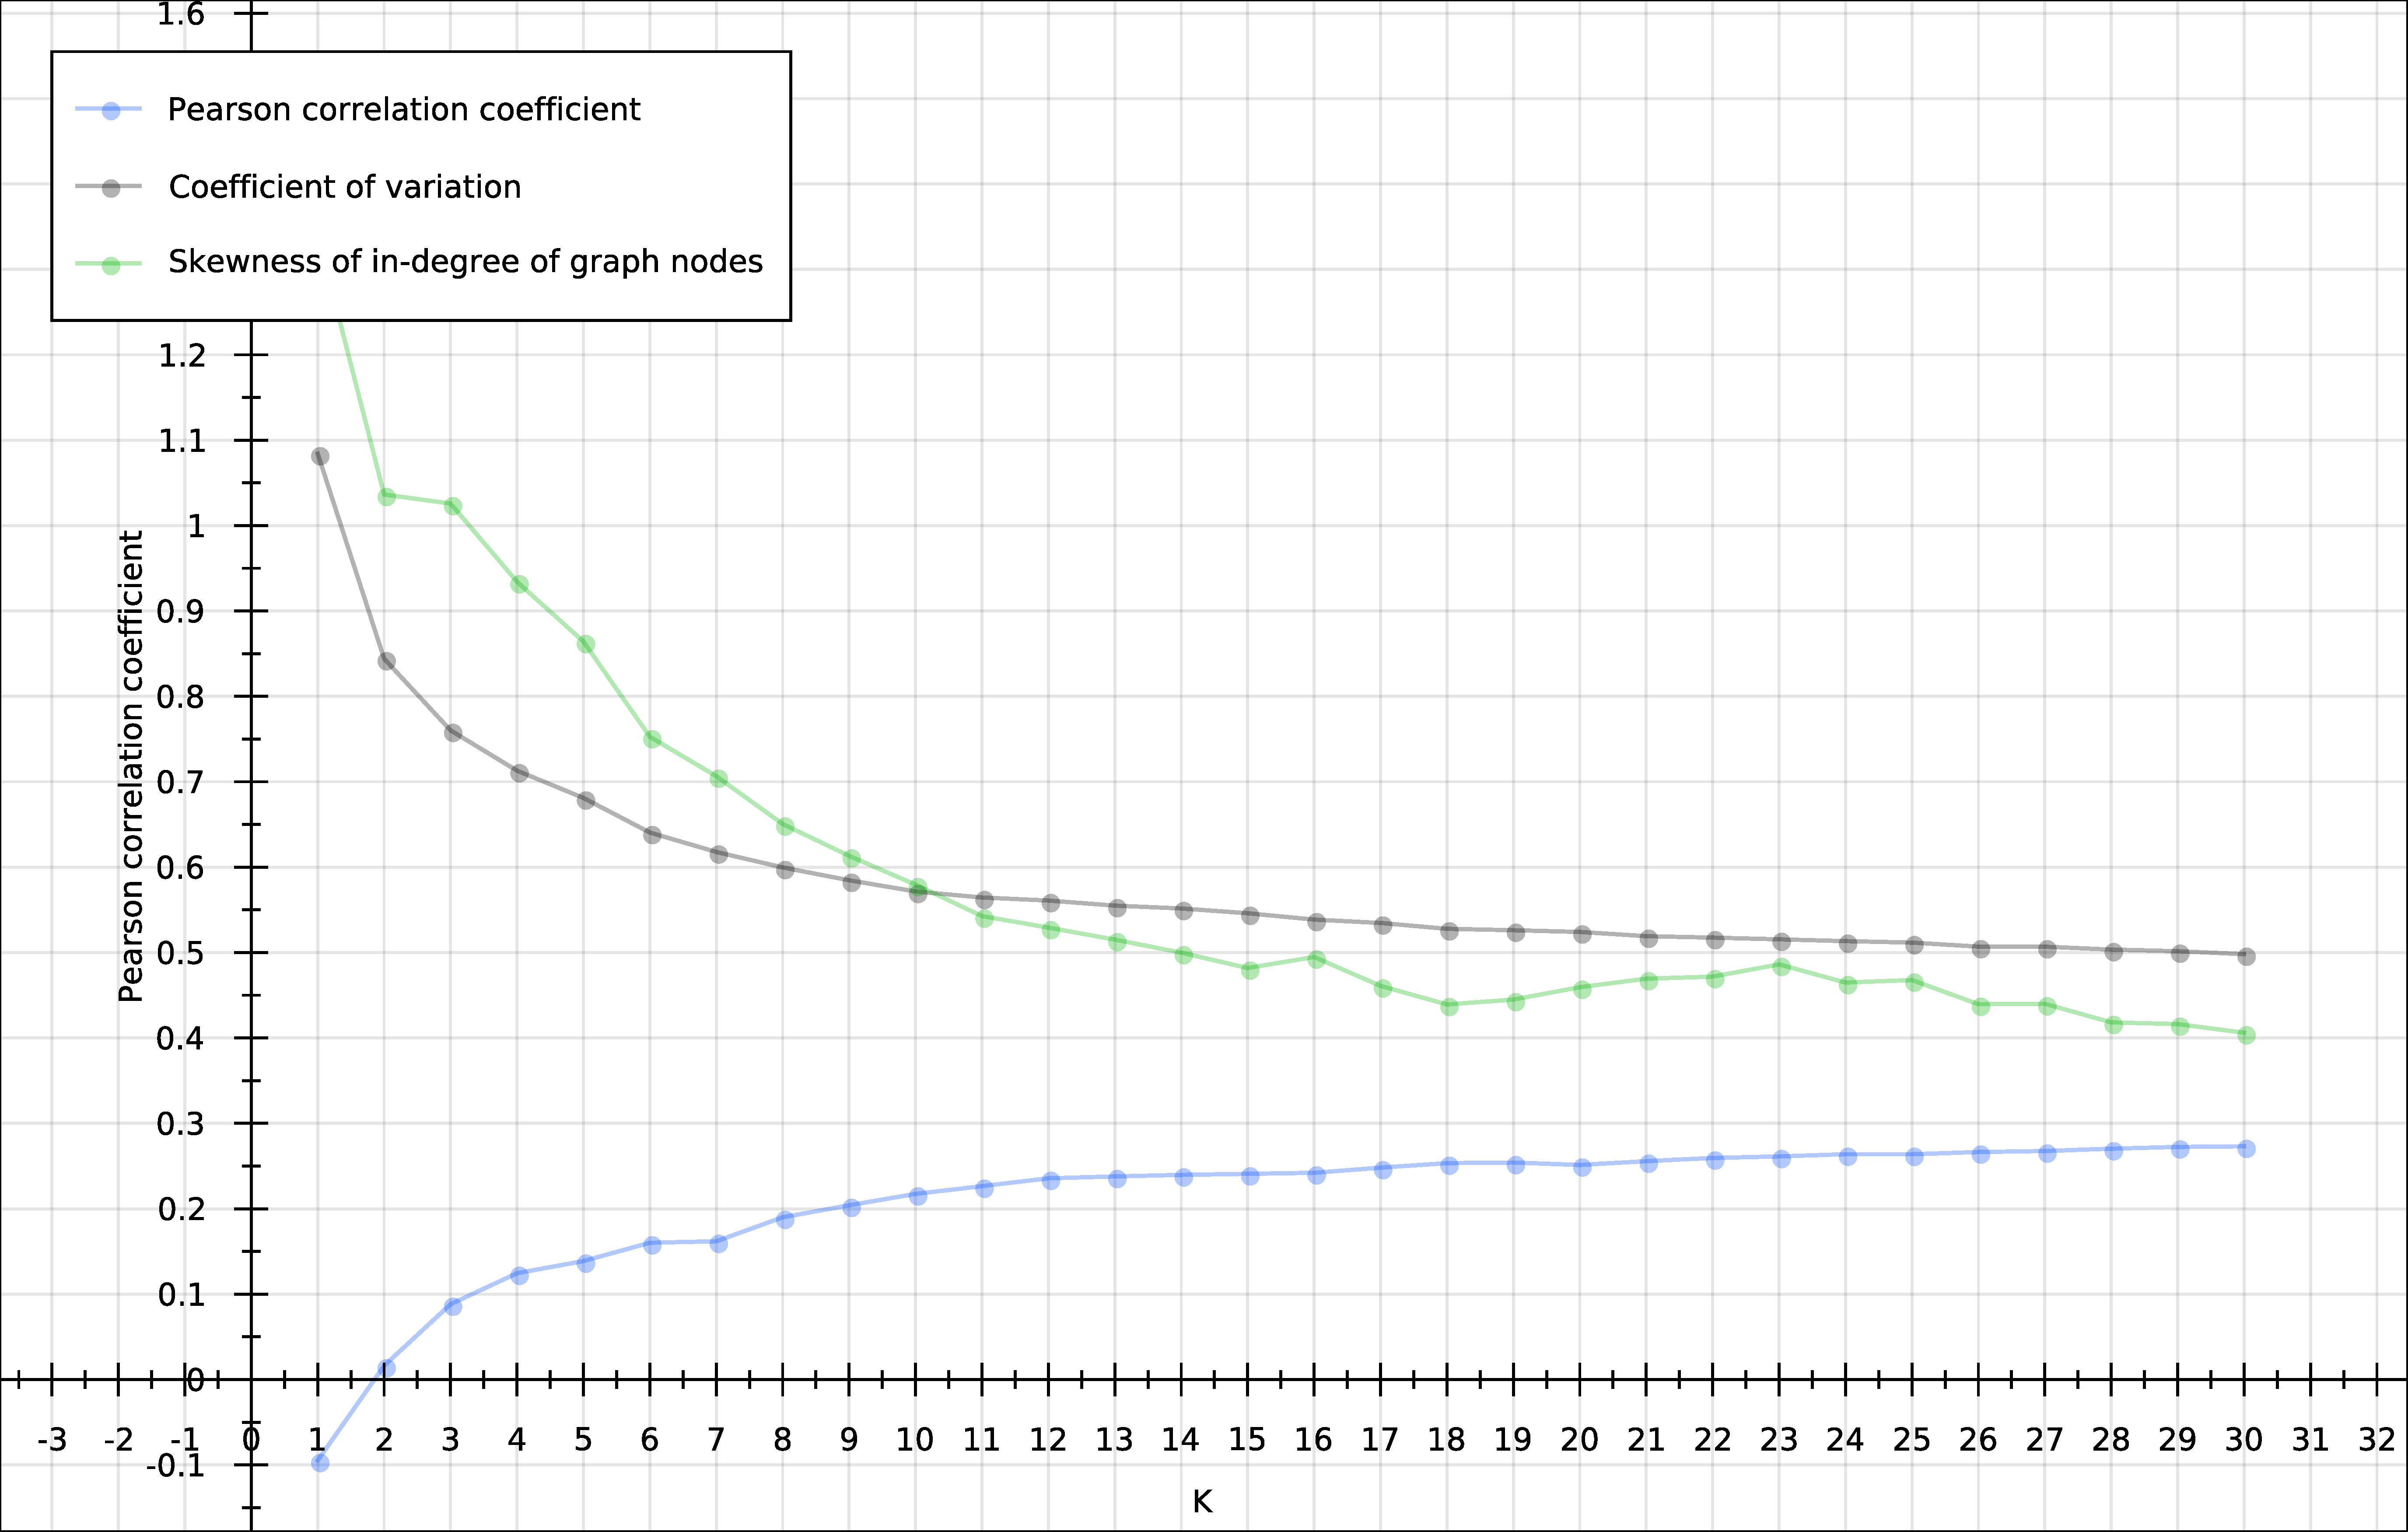
\includegraphics[width=0.95\textwidth]{images/mfeat_pearson.pdf}
  \caption{Graph of Pearson correlation coefficient, its coefficient of variation and skewness of in-degree of nodes against $K$ parameter for handwritten numerals dataset.}
  \label{fig:graph_mfeat_pearson}
\end{figure}


\clearpage
%------------------------------------------
\subsection{Steel plate faults dataset}
Steel plate faults dataset exhibits quite different parameters than 2 previous ones.
Its assortativity index stabilizes at around $0.31$ as in previous examples yet covariance of variation of nodes in-degrees descends below level of $0.3$ overlapping with assortativity index.

Skewness of nodes' in-degrees descends to negative values up until $-1.2$ for $k = 30$ indicating abence of hubness phenomena.

\begin{figure}[h!]
  \centering
  \captionsetup{justification=centering}
    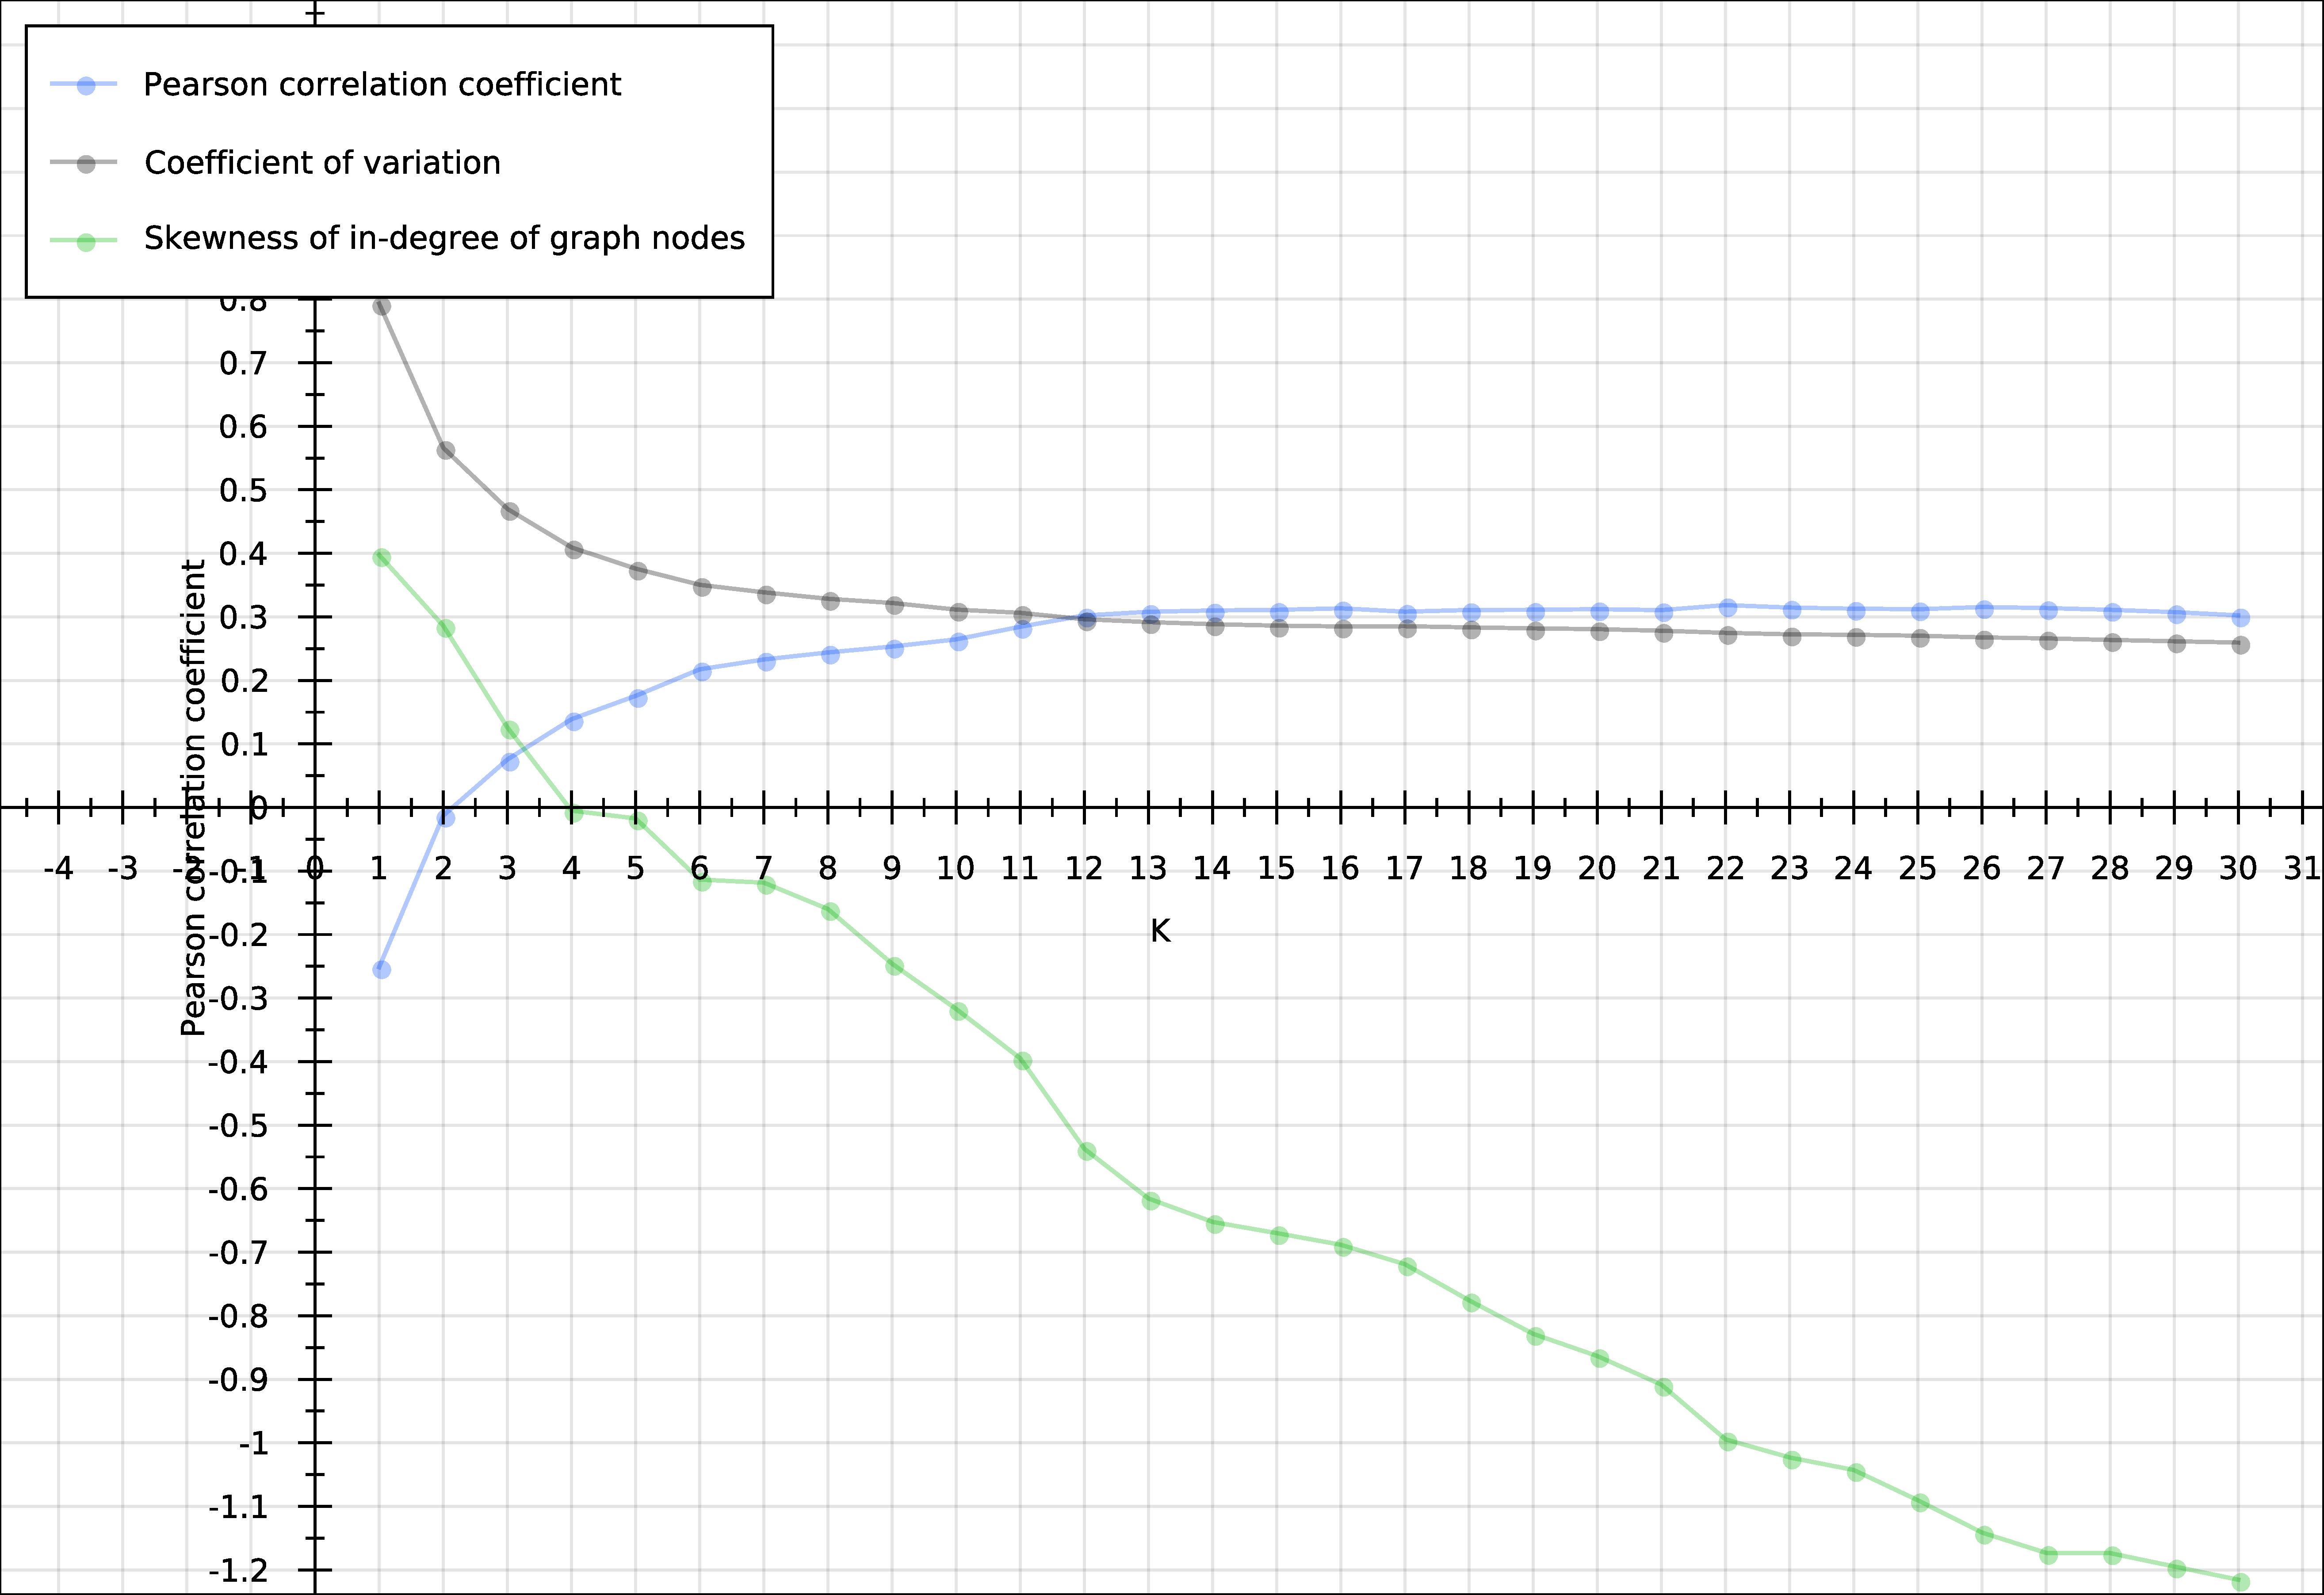
\includegraphics[width=0.95\textwidth]{images/faults_pearson.pdf}
  \caption{Graph of Pearson correlation coefficient, its coefficient of variation and skewness of in-degree of nodes against $K$ parameter for steel plates faults dataset.}
  \label{fig:graph_faults_pearson}
\end{figure}


In Figure~\ref{fig:graph_faults_nodes} one can observe tendency of nodes to connect to similar ones.
Red nodes constitute upper 25 percentile of the sample (calculated by the sume of node's values).

\begin{figure}[h!]
  \centering
  \captionsetup{justification=centering}
    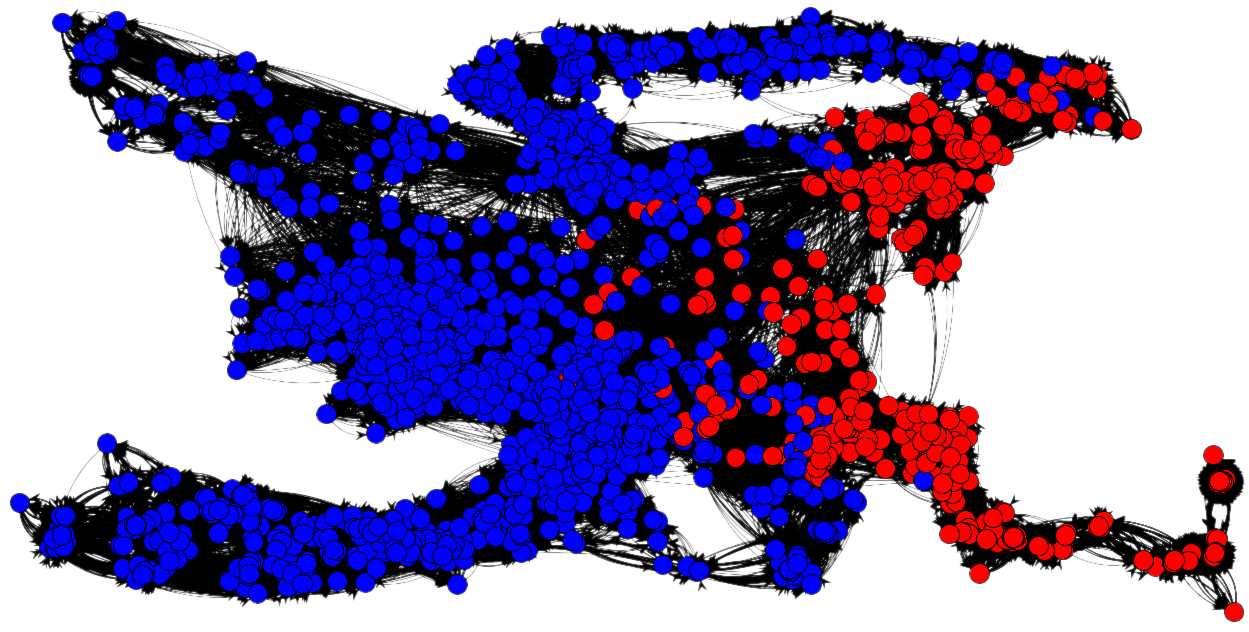
\includegraphics[width=0.95\textwidth]{images/faults_graph.png}
  \caption{K-NN graph representation of steel plates faults dataset with red nodes being the upper 25 perentile of dataset. This graph is showing medium positive assortativity coefficient of $0.30243338685364907$ which exhibits in nodes being connected to similar ones.}
  \label{fig:graph_faults_nodes}
\end{figure}

%------------------------------------------
\subsection{General conclusions}
General conclusion taken from aforementioned 3 datasets are as follows:
\begin{itemize}
\item k-NN graphs tend to be dissasortative or show no (dis)assortative mixing for small k ($k = 1$),
\item k-NN graphs tend to be assortative for large $k$,
\item assortativity for large $k$s occurs regardless of hubness phenomena ( e.g. both cardiac arrythmia dataset steel plates faults dataset positively assortative with and without hubs respectively) 
\end{itemize}




%============================================================


%\clearpage
%\section{Summary} 
%This was a paper about kNN graphs.

TO BE CHANGED.

%============================================================

\clearpage
\label{Bibliography} 
%
\bibliographystyle{siam}
\footnotesize{ \bibliography{bibliography} }
% In that case, remember to run bibtex:
% latex template; bibtex template; latex template; latex template; 

%============================================================

%\clearpage
%\begin{appendices}
%
%\section{Extending GLSurfaceView class to capture user input.}
%\label{App:Appendix_A}
%\begin{filecode}[label=lst:glsurfaceview_override]
%\lstinputlisting{./code/opengles_glsurfaceview_override.java}
%\end{filecode}
%
%\end{appendices}

\end{document}